
\section{Introduction}
The goal of the experiment is to adjust a diode laser in such a way that it causes Rubidium to fluoresce. The absorption spectrum of Rubidium is also to be recorded.
\section{Theory}
\subsection{Laser}
A Laser is a device which uses light amplification by stimulated emission of radiation. To get a laser to work we need to use population inversion and stimulated emission. The light it emitts through stimulated emission is coherent. That indicates that the photons emitted by the source have the same phase and wavelength. Since the photons have the same phase, they interfere constructively which leads to a high intensity for the laser beam.
\subsection{Spontaneous and Stimulated Emission}
If electrons in an excited energy level fall randomly into a lower energy level and emit a photon while doing so we speak about spontaneous emission. The photon created by this has a random direction and polarization and this is unpreferable for this experiment. That is why stimulated emission is needed. Stimulated emission is the process of radiating a photon of a specific direction and wavelength. That can be done by exciting an electron to a higher energy level with a photon with the needed properties. A laser is operating with this stimulated emission, because it can generate coherent light. For a laser to use stimulated emission population inversion is needed.
\subsection{Population Inversion}
Population inversion means that more electrons of a system are in a higher energy level compared to the ones in the ground state. This is necessary for stimulated emission because otherwise the system would be more prone to spontaneous emission. To understand population inversion a discussion of the thermal distribution by Boltzmann is needed. \\
The relation 
\begin{equation*}
    \frac{N_2}{N_1}=\exp \left(\frac{-(E_2 - E_1)}{k_B T}\right),
\end{equation*}
with $N_i$ being the electron densities of the differing states, $k_B$ being the Boltzmann constant and $T$ being the temperature, shows that $\frac{N_2}{N_1} < 1$ because of $E_2$ being larger than $E_1$. Boltzmann implies that in thermal equilibrium more electrons reside in the ground state than in higher energy states. For population inversion it is needed to invert that predicate. \\
The inversion is not possible with a two level system as shown above so a three level system is needed. The excitation of the electrons which is also called pump can be done by the absorption of a photon for example. If the pumping is rapid the energy density ration becomes $\frac{N_3}{N_1}=1$ with $N_3$ being the electron density of the energy $E_3$ from the third energy level the ground state electrons are pumped into. The electrons in the third energy level $E_3$ will transition into the second energy level $E_2$ by some transition time $t_{32} < t_{21}$. This means that more electrons will be in the energy state with $E_2$ than in the ground state with $E_1$. Because energy is constantly put into the ground states there cannot be spontaneous emission and only stimulated emission as desired.
\subsection{Diode Laser}
Diodes consist of two types of differently doted semiconducters. They contain a barrier layer between a n-(negative) doped part and a p-(positive) doped part. This is called the n-p-junction. By applying a certain voltage with the correct polarity the electrons flow to the transmission direction. This leads to a recombination of the elctron-hole-pairs. This emits energy equal to the band gap which seperates the valence and conduction band and emits also therefore a photon. There is a threshold for stimulated emission and under this threshold only spontaneous emission is happening. By raising the injection current the energy needed to jump over the band gap is elevated resulting in a larger wavelength.\\
\begin{figure}[H]
    \centering
    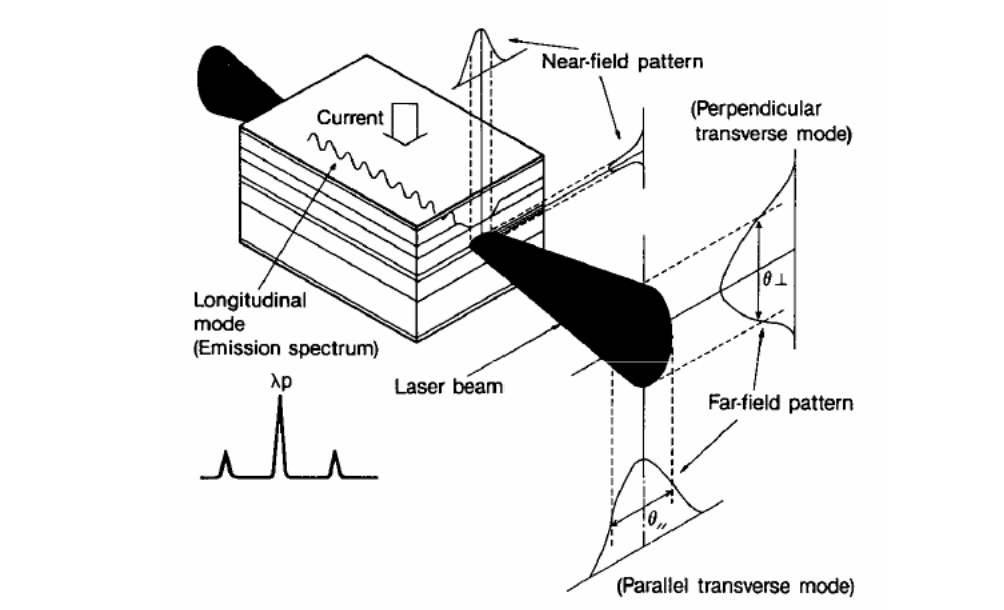
\includegraphics[width=10cm]{content/active_layer.png}
    \caption{The active layer of a diode laser.}
\end{figure}
The active layer in the chip inside the diode laser works like a Fabry-pelot etalon. This is a cavity with a reflective layer at the front and back facet. The back facet is highly reflective and the front facet semipermeable and the laser beam transmitts divergent from it. The divergence can be bypassed by a collimating lens.\\
The length of the internal cavity of the diode laser sets the periodicy of the maximum of the net gain depending on the wavelength of the light emitted. To shorten the spectral width a diffraction grating is added.\\
\begin{figure}[H]
    \centering
    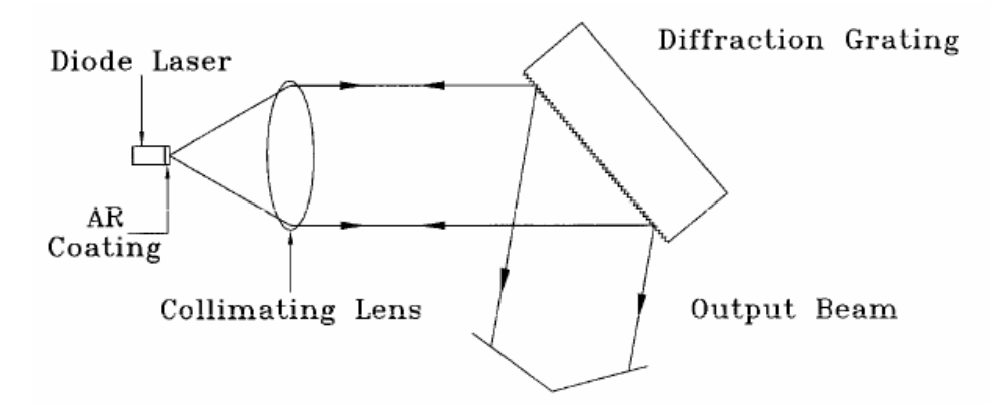
\includegraphics[width=10cm]{content/external_cavity.png}
    \caption{The external cavity of a diode laser.}
\end{figure}
This external cavity works like the internal cavity with the difference that maximum overall gain is available for many more wavelengths because the free spectral width gets smaller because of the grating. The diffraction grating feedbacks the desired wavelength through the Bragg equation
\begin{equation}
    n\lambda=2d\sin(\theta)
\end{equation}
with the order of diffraction $n$, the incident wavelength $\lambda$ the grid spacing $d$ of the crystal used and the angle of incidence $\theta$.\\
\begin{figure}[H]
    \centering
    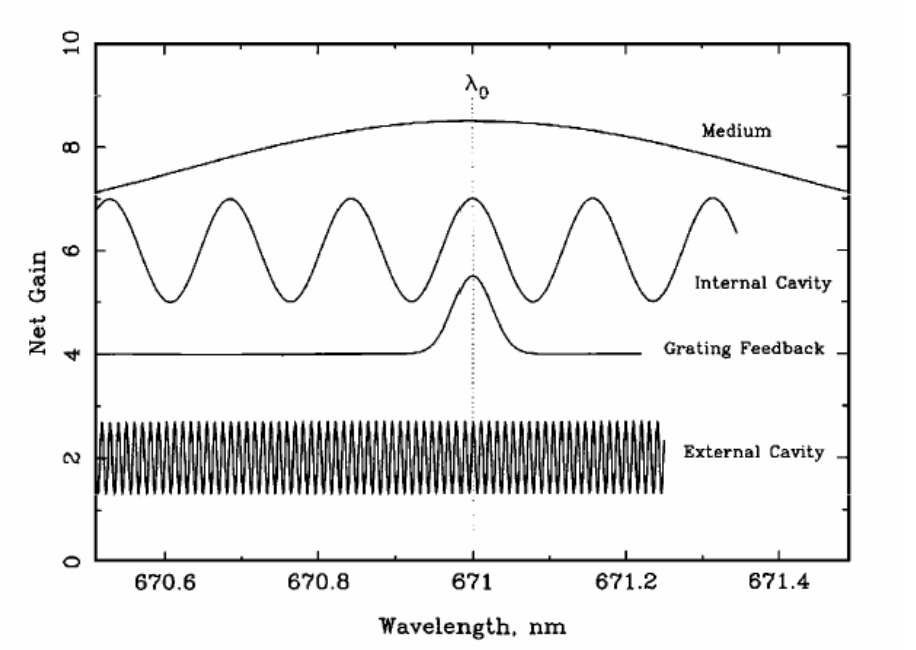
\includegraphics[width=10cm]{content/net_gain.png}
    \caption{The net gain graph of a diode laser.}
\end{figure}
The net gain contributions of the medium, the internal cavity, the diffraction grating and the external cavity multiply and amplify the adjusted wavelength.\\
\begin{figure}[H]
    \centering
    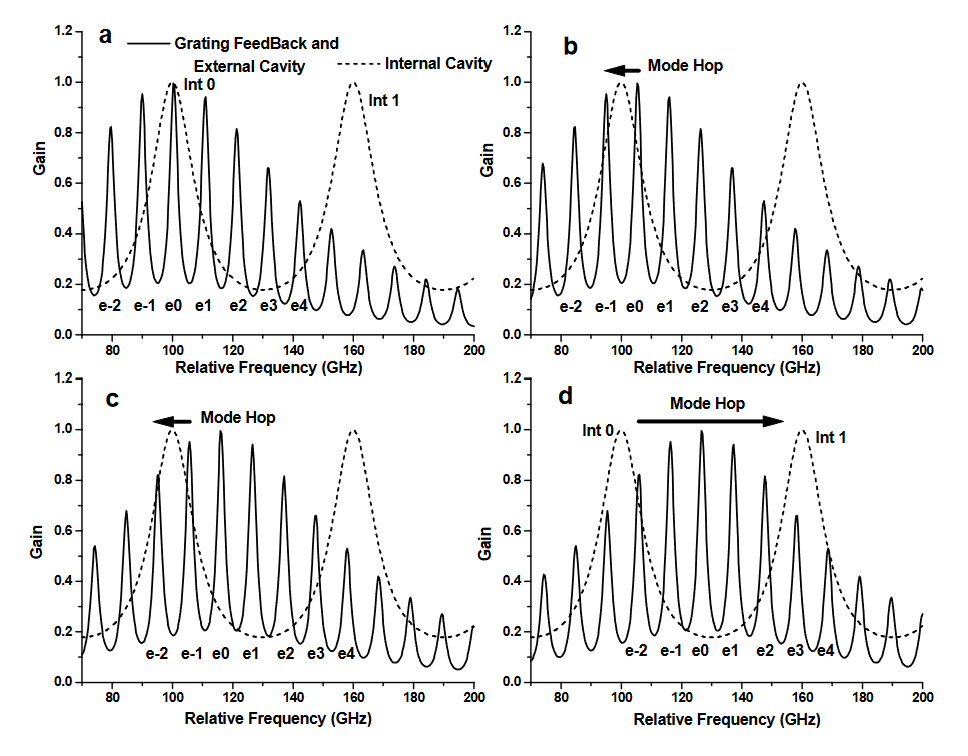
\includegraphics[width=10cm]{content/mode_hop.png}
    \caption{Graph of mode hops in a diode laser.}
\end{figure}
The laser mode of the laser diode can be varied by changing the angle of the diffraction grating. Varying the angle can cause laser mode hops, because the net gain function of the internal cavity has less maxima while the external one has more. Moving the net gain curve of the external cavity by changing the angle inside the next maxima of the internal cavity causes these mode hops.
\subsection{Rubidium Fluorescence}
Fluroscence is the emission of light by an atom through the relase of a photon by an electron jumpng from an excited state to a lower energy state. Rubidium has the electron configuration [Kr] $5s^1$ which means that only the electrons of the $5s$ shell can be excited. This can be done by a laser with a wavelength of 780 nm. There are two energy transitions which emitt light. Four transitions are possible in this experiment, because Rubidium appears naturally in the combination of $^{85}$Rb and $^{87}$Rb.
\begin{figure}[H]
    \centering
    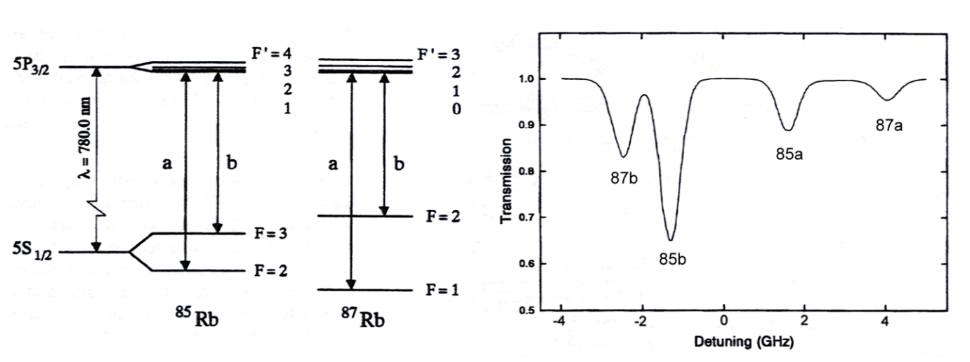
\includegraphics[width=10cm]{content/rubidium_flourescence.png}
    \caption{Diagram of energy levels and absorption spectrum of rubidium.}
\end{figure}
\section{Experimental Setup}
\subsection{Detecting the lasing threshold}
To detect the lasing threshold an IR-Card is used. This card makes infrared light (700 nm - 1350 nm) visible. This card is placed in a card holder right in front of the laser. Because the light is just little visible on the card, a ccd camera is used which makes the light fully visible. Because of spontanious emission the laser first operates like a LED. Only when sprinkles are visible the laser operates as a laser. This happens in a jump and the current induced is the current threshold of the laser.
\begin{figure}[H]
    \centering
    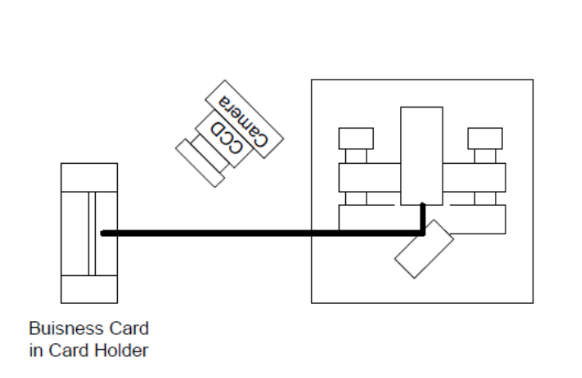
\includegraphics[width=10cm]{content/exp1.png}
    \caption{Diagram of the threshold setup.}
\end{figure}
\subsection{Observing Rubidium fluorescence}
A heated Rubidium gas chamber is placed in front of the laser. A ccd camera is place on the side of the gas chamber to make the flourescence visible because the laser has to hit the gas with a wavelength of 780 nm. The laser doesn't start with a wavenlength of 780 nm. The grating and current is to adjust to get the laser to operate on a wavenlength of 780 nm. The flourescence can be seen horizontaly on the ccd camera after the wavenelgth is found.
\begin{figure}[H]
    \centering
    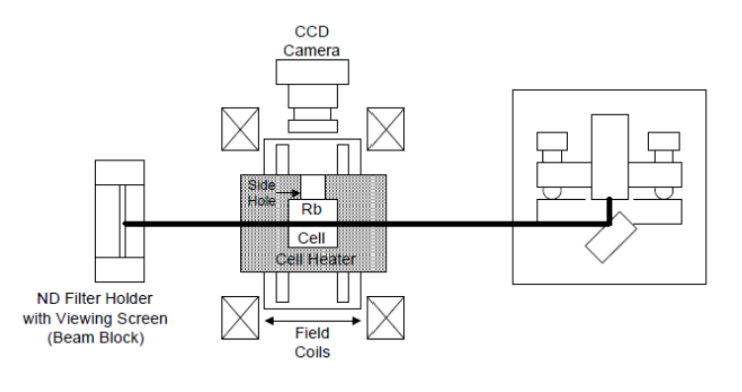
\includegraphics[width=10cm]{content/exp2.png}
    \caption{Diagram of the flourescence setup.}
\end{figure}
\subsection{Measuring the Rubidium absorption}
 The laser beam is splitted into two beams using a semi-permeable 50/50-mirror. Both beams enter a photodiode. The first photodiode is used to adjust the graph later on because the current is sweeped. Both photodiodes are connected to an oscilloscope which is to adjust to get the absorption spectrum of Rubidium. 
 \begin{figure}[H]
    \centering
    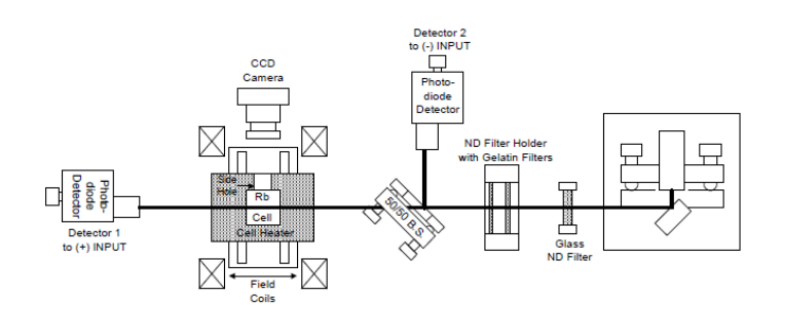
\includegraphics[width=10cm]{content/exp3.png}
    \caption{Diagram of the absorption setup.}
\end{figure} 
